% Options for packages loaded elsewhere
% Options for packages loaded elsewhere
\PassOptionsToPackage{unicode}{hyperref}
\PassOptionsToPackage{hyphens}{url}
\PassOptionsToPackage{dvipsnames,svgnames,x11names}{xcolor}
%
\documentclass[
  letterpaper,
  DIV=11,
  numbers=noendperiod]{scrartcl}
\usepackage{xcolor}
\usepackage{amsmath,amssymb}
\setcounter{secnumdepth}{-\maxdimen} % remove section numbering
\usepackage{iftex}
\ifPDFTeX
  \usepackage[T1]{fontenc}
  \usepackage[utf8]{inputenc}
  \usepackage{textcomp} % provide euro and other symbols
\else % if luatex or xetex
  \usepackage{unicode-math} % this also loads fontspec
  \defaultfontfeatures{Scale=MatchLowercase}
  \defaultfontfeatures[\rmfamily]{Ligatures=TeX,Scale=1}
\fi
\usepackage{lmodern}
\ifPDFTeX\else
  % xetex/luatex font selection
\fi
% Use upquote if available, for straight quotes in verbatim environments
\IfFileExists{upquote.sty}{\usepackage{upquote}}{}
\IfFileExists{microtype.sty}{% use microtype if available
  \usepackage[]{microtype}
  \UseMicrotypeSet[protrusion]{basicmath} % disable protrusion for tt fonts
}{}
\makeatletter
\@ifundefined{KOMAClassName}{% if non-KOMA class
  \IfFileExists{parskip.sty}{%
    \usepackage{parskip}
  }{% else
    \setlength{\parindent}{0pt}
    \setlength{\parskip}{6pt plus 2pt minus 1pt}}
}{% if KOMA class
  \KOMAoptions{parskip=half}}
\makeatother
% Make \paragraph and \subparagraph free-standing
\makeatletter
\ifx\paragraph\undefined\else
  \let\oldparagraph\paragraph
  \renewcommand{\paragraph}{
    \@ifstar
      \xxxParagraphStar
      \xxxParagraphNoStar
  }
  \newcommand{\xxxParagraphStar}[1]{\oldparagraph*{#1}\mbox{}}
  \newcommand{\xxxParagraphNoStar}[1]{\oldparagraph{#1}\mbox{}}
\fi
\ifx\subparagraph\undefined\else
  \let\oldsubparagraph\subparagraph
  \renewcommand{\subparagraph}{
    \@ifstar
      \xxxSubParagraphStar
      \xxxSubParagraphNoStar
  }
  \newcommand{\xxxSubParagraphStar}[1]{\oldsubparagraph*{#1}\mbox{}}
  \newcommand{\xxxSubParagraphNoStar}[1]{\oldsubparagraph{#1}\mbox{}}
\fi
\makeatother


\usepackage{longtable,booktabs,array}
\usepackage{calc} % for calculating minipage widths
% Correct order of tables after \paragraph or \subparagraph
\usepackage{etoolbox}
\makeatletter
\patchcmd\longtable{\par}{\if@noskipsec\mbox{}\fi\par}{}{}
\makeatother
% Allow footnotes in longtable head/foot
\IfFileExists{footnotehyper.sty}{\usepackage{footnotehyper}}{\usepackage{footnote}}
\makesavenoteenv{longtable}
\usepackage{graphicx}
\makeatletter
\newsavebox\pandoc@box
\newcommand*\pandocbounded[1]{% scales image to fit in text height/width
  \sbox\pandoc@box{#1}%
  \Gscale@div\@tempa{\textheight}{\dimexpr\ht\pandoc@box+\dp\pandoc@box\relax}%
  \Gscale@div\@tempb{\linewidth}{\wd\pandoc@box}%
  \ifdim\@tempb\p@<\@tempa\p@\let\@tempa\@tempb\fi% select the smaller of both
  \ifdim\@tempa\p@<\p@\scalebox{\@tempa}{\usebox\pandoc@box}%
  \else\usebox{\pandoc@box}%
  \fi%
}
% Set default figure placement to htbp
\def\fps@figure{htbp}
\makeatother





\setlength{\emergencystretch}{3em} % prevent overfull lines

\providecommand{\tightlist}{%
  \setlength{\itemsep}{0pt}\setlength{\parskip}{0pt}}



 


\KOMAoption{captions}{tableheading}
\makeatletter
\@ifpackageloaded{caption}{}{\usepackage{caption}}
\AtBeginDocument{%
\ifdefined\contentsname
  \renewcommand*\contentsname{Table of contents}
\else
  \newcommand\contentsname{Table of contents}
\fi
\ifdefined\listfigurename
  \renewcommand*\listfigurename{List of Figures}
\else
  \newcommand\listfigurename{List of Figures}
\fi
\ifdefined\listtablename
  \renewcommand*\listtablename{List of Tables}
\else
  \newcommand\listtablename{List of Tables}
\fi
\ifdefined\figurename
  \renewcommand*\figurename{Figure}
\else
  \newcommand\figurename{Figure}
\fi
\ifdefined\tablename
  \renewcommand*\tablename{Table}
\else
  \newcommand\tablename{Table}
\fi
}
\@ifpackageloaded{float}{}{\usepackage{float}}
\floatstyle{ruled}
\@ifundefined{c@chapter}{\newfloat{codelisting}{h}{lop}}{\newfloat{codelisting}{h}{lop}[chapter]}
\floatname{codelisting}{Listing}
\newcommand*\listoflistings{\listof{codelisting}{List of Listings}}
\makeatother
\makeatletter
\makeatother
\makeatletter
\@ifpackageloaded{caption}{}{\usepackage{caption}}
\@ifpackageloaded{subcaption}{}{\usepackage{subcaption}}
\makeatother
\usepackage{bookmark}
\IfFileExists{xurl.sty}{\usepackage{xurl}}{} % add URL line breaks if available
\urlstyle{same}
\hypersetup{
  colorlinks=true,
  linkcolor={blue},
  filecolor={Maroon},
  citecolor={Blue},
  urlcolor={Blue},
  pdfcreator={LaTeX via pandoc}}


\author{}
\date{}
\begin{document}


\section{La poliarquía}\label{poliarquia}

\begin{quote}
Reporte de lectura:

Dahl, Robert Alan. «La poliarquía.» En \emph{Diez textos básicos de
ciencia política}, de Albert Batlle Rubio, 77-92. Barcelona, España:
Ariel, 1992.

* Ed. original: R. A. Dahl, \emph{A Preface to Democratic Theory}, cap.
3, The University of Chicago Press, 1956.
\end{quote}

\subsection{Síntesis}\label{suxedntesis}

Dahl plantea que la democracia es una utopía, un ideal que los estados,
que se denominan democráticos, aspiran a alcanzar; un ideal donde hay
perfecta igualdad política y soberanía popular; por lo que sostiene que
en la práctica los estados ``democráticos'' tienden a ser regímenes
poliárquicos. La definición de estos regímenes la desarrolla al buscar
maximizar el \emph{gobierno del pueblo} (soberanía popular e igualdad
política), lo que resulta en el establecimiento de ocho condiciones que
podrían ser vistas como una definición operativa de democracia.

\subsection{Tesis}\label{tesis}

Al presuponer que la democracia, en su definición teórica, es una
utopía, Dahl plantea las siguientes condiciones que se deberían alcanzar
para, en la realidad, tratar de lograr un gobierno del pueblo:

\begin{enumerate}
\def\labelenumi{\arabic{enumi}.}
\item
  Derecho a la expresión de preferencias (p.e. derecho al voto).
\item
  El peso de la elección de cada individuo es idéntico.
\item
  La alternativa más seleccionada es la ganadora.
\item
  Cualquiera que perciba un conjunto de alternativas, y considere al
  menos una de ellas preferible a las demás, puede añadirla a las
  seleccionadas para la votación.
\item
  Todos poseen idéntica información sobre las alternativas.
\item
  Las alternativas con más votos desplazan a las que tienen menos votos.
\item
  Las ordenes de los cargos electos se cumplen.
\item
  Las nuevas decisiones del período interelectoral están regidas por las
  condiciones precedentes; o que las decisiones interelectorales están
  subordinadas a las establecidas durante la etapa de elección o que son
  aplicación de éstas.
\end{enumerate}

\subsection{Ideas secundarías}\label{ideas-secundaruxedas}

\begin{itemize}
\item
  La poliarquía no es ni un gobierno de mayoría pura ni un gobierno
  unificado de una minoría. Es un sistema abierto, competitivo y
  pluralista de gobierno de minorías.
\item
  El nivel de poliarquía existente dependerá de la medida en que se
  consideren deseables las ocho condiciones.
\item
  La poliarquía es una función de la actividad política de los miembros.
\item
  El nivel de instrucción social en una de las ocho condiciones aumenta
  también con el grado de acuerdo existente sobre ella.
\end{itemize}

\subsection{Reflexión}\label{reflexiuxf3n}

Leyendo el texto de Dahl desde la perspectiva de la teoría de la clase
política de Mosca, pareciera que ``la poliarquía es una negociación
entre minorías organizadas'' {[}@krouse1982{]} inmersas en una mayoría
desorganizada, dando pie a un ``juego democrático'' {[}@bovero1998{]}
que busca maximizar el consenso y minimizar la imposición bajo las
reglas democráticas; donde la ``efectividad política de cada grupo
estaría en función de su potencial de control y de unidad''
{[}@dahl1958{]}.

Desde un punto de vista práctico, la propuesta de Dahl puede brindar una
escala medible para ver qué tan cerca un estado o institución se
encuentra de ser democrático (poliárquico); y, aunque las condiciones o
normas planteadas no dan de manera operativa un camino para alcanzar la
democracia, en su definición ideal, sí permiten plantear objetivos
reales para acercarse a estados más democráticos.

Actualmente, El Economista plantea un índice
{[}@theeconomistintelligenceunit2025{]}, que mide la democracia de los
países usando cinco categorías: Libertades civiles, Participación
Política, Proceso electoral y pluralismo, Funcionamiento del gobierno y
Cultura política; de acuerdo con los resultados, clasifica a los países
en cuatro categorías que van de Democracias completas a Regímenes
autoritarios. En 2024, ubicó a México como un régimen Hibrido, además ha
mantenido una tendencia a la baja desde 2013, ver Figura 1. La IDEA, por
su parte, plantea cuatro índices para medir el estado de la democracia
{[}@internationalinstitutefordemocracyandelectoralassistance2025{]}:
Representación, Derechos, Participación y Estado de Derecho; en 2024
resaltó que el índice que México tiene más bajo es el de Estado de
Derecho, con 0.36 en una escala de 0-1; debido a que este índice tiene
un subíndice que mide la independencia del poder judicial.

\begin{center}
\pandocbounded{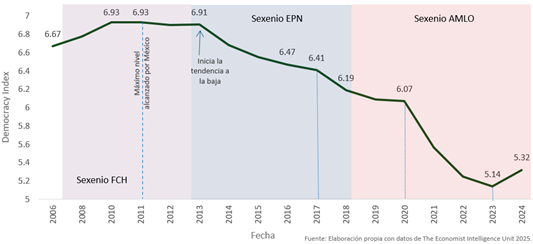
\includegraphics[keepaspectratio]{./www/08_poliarquia.png}}
\end{center}




\end{document}
